\chapter{Background}\label{background}

    This chapter aim to explain technologies, tools, and specification of a device that are used in this project.
    Then, this chapter gives an analysis of related applications.

    \section{Threading in Android}
        Threads in Android development are categorised into 2 main categories: a main thread and a worker thread.
        A main thread or UI thread is a thread that dispatch events of user interface widgets.
        The events is dispatched regarding to Android's activity lifecycle,
        and all events are managed by only 1 thread.
        In other words, threads will not be spawned for handling a single event or component.
        Thus, if there is a long-running task, which is run by UI thread, events cannot be delivered.
        In addition, an application will show "Application not Responding"
        when UI thread is blocked more than 5 seconds \cite{ANDROID-01}.

        \begin{figure}[!ht]
            \centering
            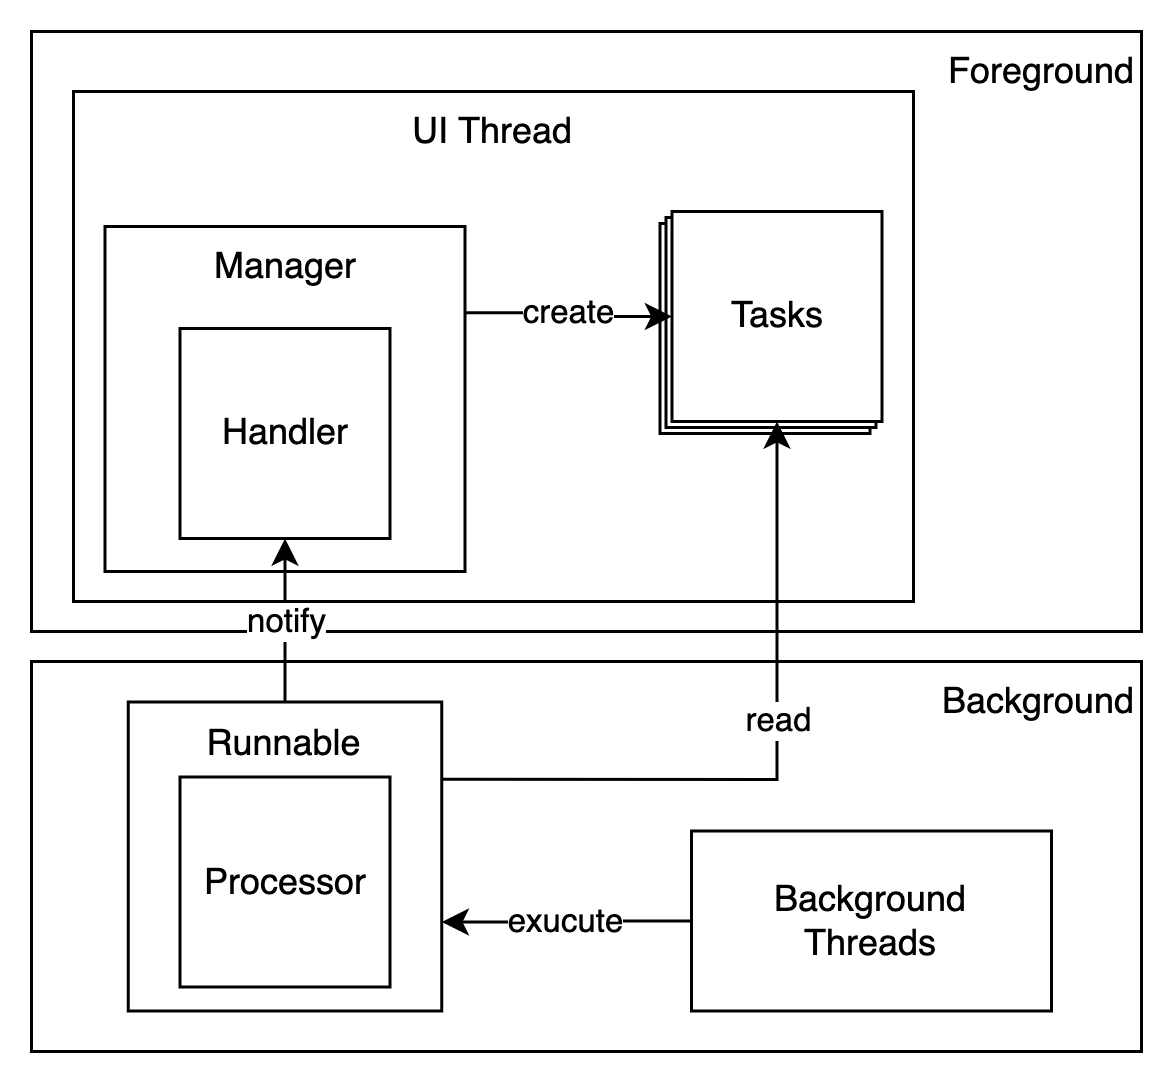
\includegraphics[width=4in]{images/chapter2/thread-overview.png}
            \caption{Threading Overview}
            \label{thread-overview}
        \end{figure}

        To avoid freezing application, a working thread is separated from the UI thread,
            and it is called worker thread or background thread.
            This thread is able to process a long-running task in the background without interrupting the UI thread.
        In addition, the priority of the thread can be set from -20 to 19--- -20
            is the highest priority, and 19 is the lowest priority.
            The default value of background threads priority is 10,
            and the default value of foreground threads is -2.

        UI thread and background thread are running on different threads;
        thus, handler is needed when there is communication between these threads.

        as shown in figure \ref{thread-overview}

        - Background thread communicate with UI thread
            - handler


    \section{Object Detection}
        -	People Detection
            - Using DNN
            - What is DNN
            - How it works
            - How it works in this project
                - Insert diagram of DNN (Flow of Image Processing)
                    - blobFronImage
                    - forward
                    - ...

    \section{Distance Calculation}\label{sectionDistanceCalculation}
        According to Gurucharan \cite{SOCIAL-DISTANCING-DETECTION}, to measure a distance between 2 people, the reference point of people are used for calculation.
        The reference point is the coordination of each people, which is the centre of the detection frame.
        The calculation formula is based on Euclidean distance.

        \begin{equation*}
            d = \sqrt{(a_{0}-b_{0})^{2}+(D/c)\times(a_{1}-b_{1})^{2}}
        \end{equation*}

        \begin{equation*}
            c = \frac{a_{1}+b_{1}}{2}
        \end{equation*}

        However, three-dimensional space are captured into two-dimensional image,
        so depth and perspective are concerned as can be seen in figure \ref{distanceCalculation}.
        Thus, a couple variables are added into the formula.
        The first variable is $D$, which is the diagonal of the image.
        The second variable is $c$, which is a calibration.
        These 2 variables will determine the depth of people in the image.

        \begin{figure}
            \centering
            \begin{subfigure}{.5\textwidth}
              \centering
              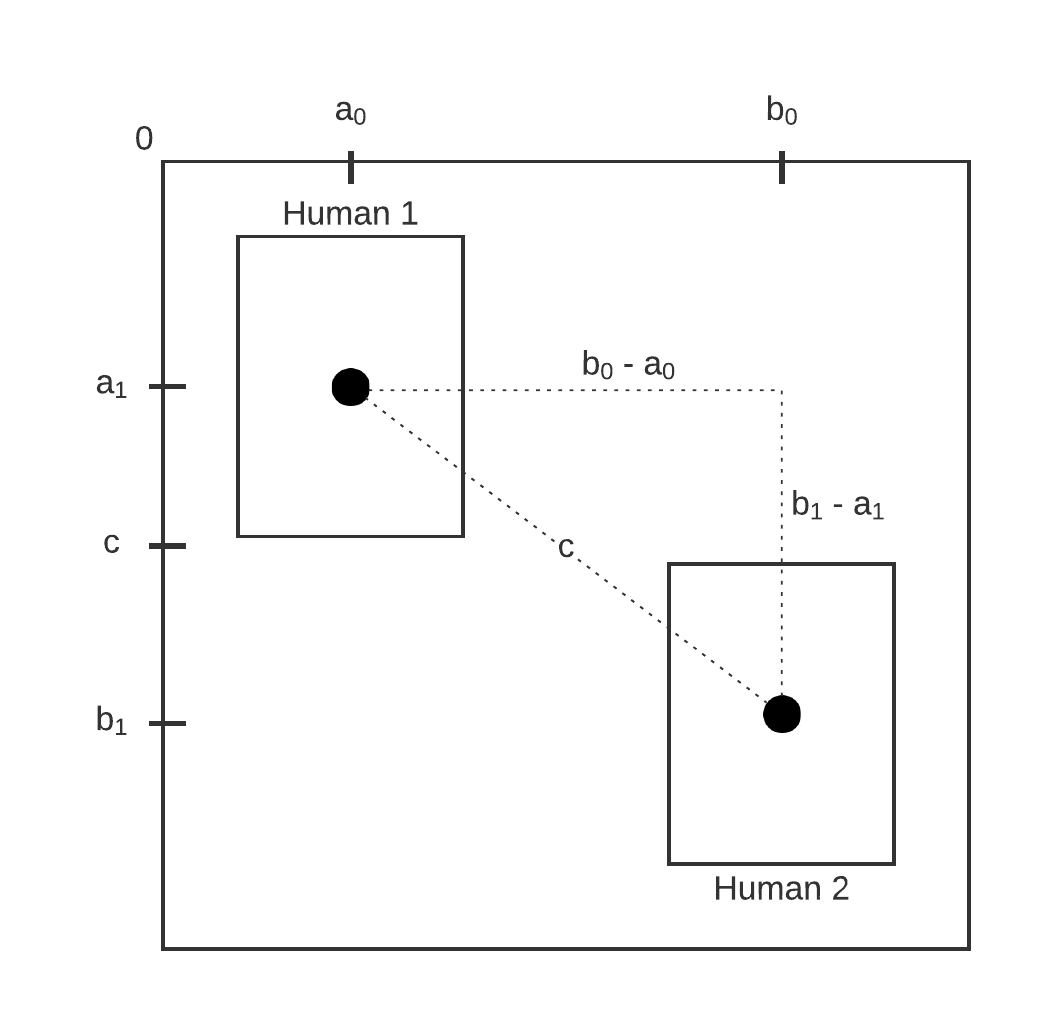
\includegraphics[width=3in]{images/chapter2/distance.png}
              \caption{Distance calculation}
              \label{distanceCalculation}
            \end{subfigure}%
            \begin{subfigure}{.5\textwidth}
              \centering
              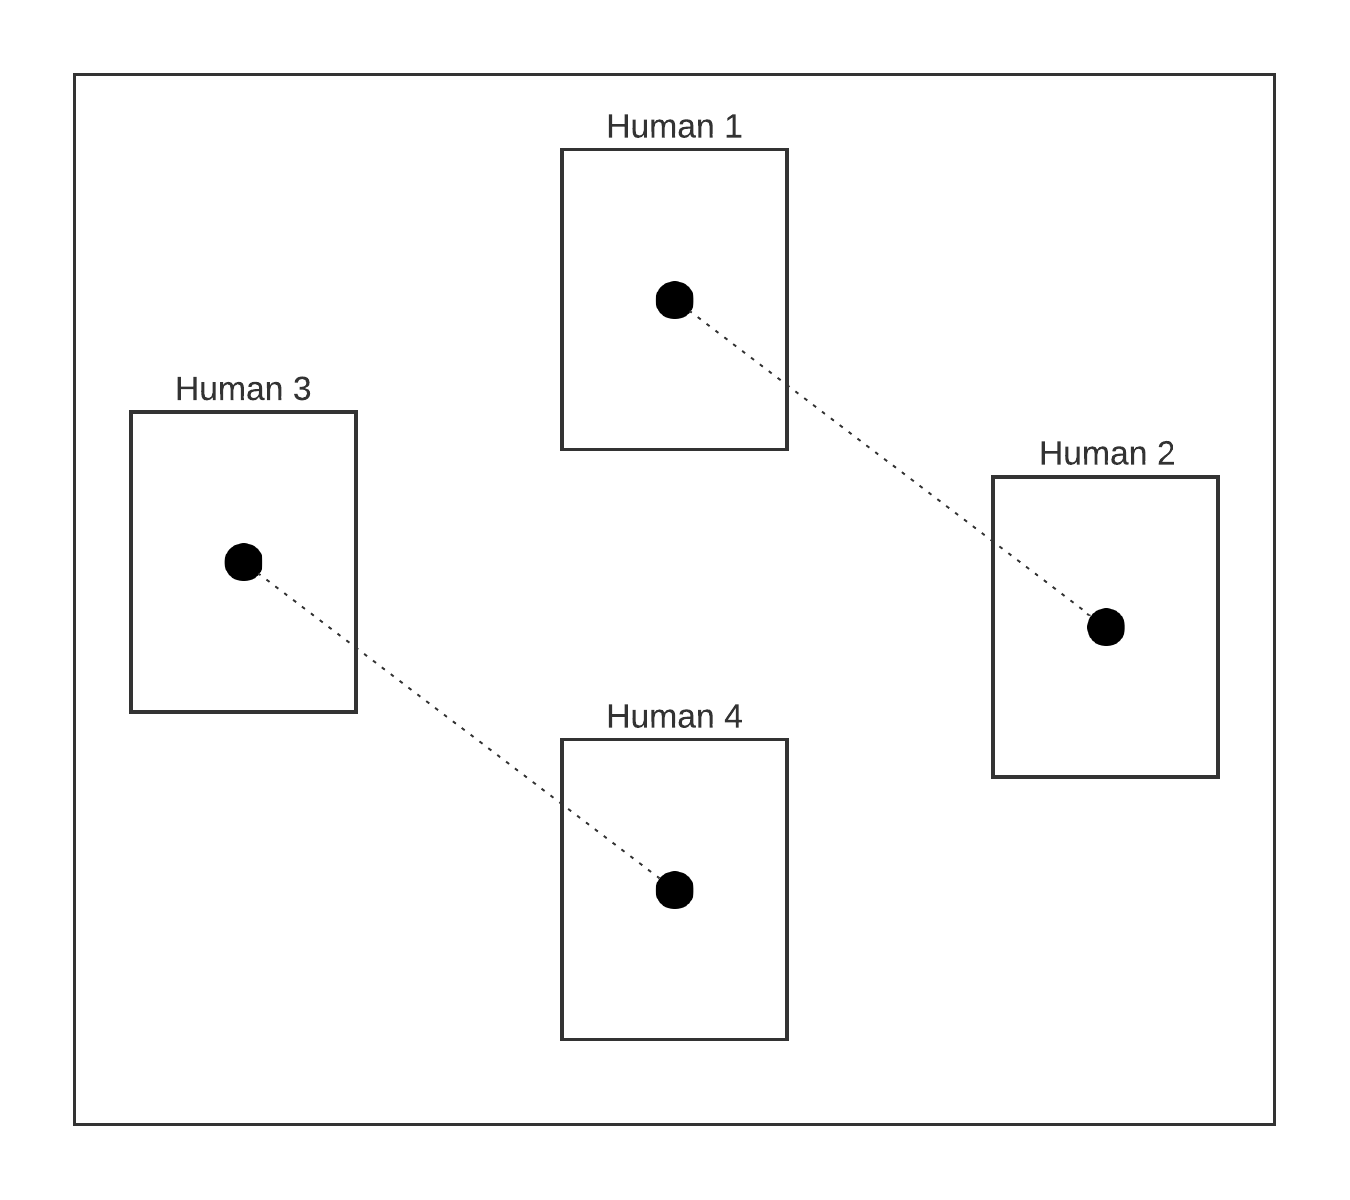
\includegraphics[width=3in]{images/chapter2/two-distances.png}
              \caption{A difference of 2 distances}
              \label{twoDistances}
            \end{subfigure}
            \caption{Determining Social Distancing}
            \label{determiningConcept}
        \end{figure}

        For example, according to the figure \ref{twoDistances},
        if distance is calculated without calibration, distance between 2 couples will be the same.
        Naturally, the distance between Human1 and Human2 must be further than the distance between Human3 and Human4.

    \section{Specification}
        This application is developed and tested on following specification:

        \begin{table}[!htp]\centering
            \caption{Specification}\label{tab: }
            \scriptsize
            \begin{tabular}{lrll}\toprule
                Device              &Device             &Samsung S10+ \\ \hline
                Operating System    &Operating System   &Android 10 (Q) \\ \hline
                Processor           &CPU                &Samsung Exynos 9820 \\
                                    &Cores              &8 \\
                                    &Architecture       &2x ARM Cortex-A75 2.73GHz \\
                                    &                   &4x ARM Cortex-A55 1.95GHz \\
                                    &                   &2x Samsung Exynos M4 1.95 GHz \\
                                    &GPU                &Mali-G76 \\ \hline
                Memory              &RAM                &8 GB \\
                \bottomrule
            \end{tabular}
        \end{table}


    \section{Existing Applications}
        \subsection{Object Detector}

            - Model: MobileNet SSD
            - Library TensorFlow

            \begin{figure}[!ht]
                \centering
                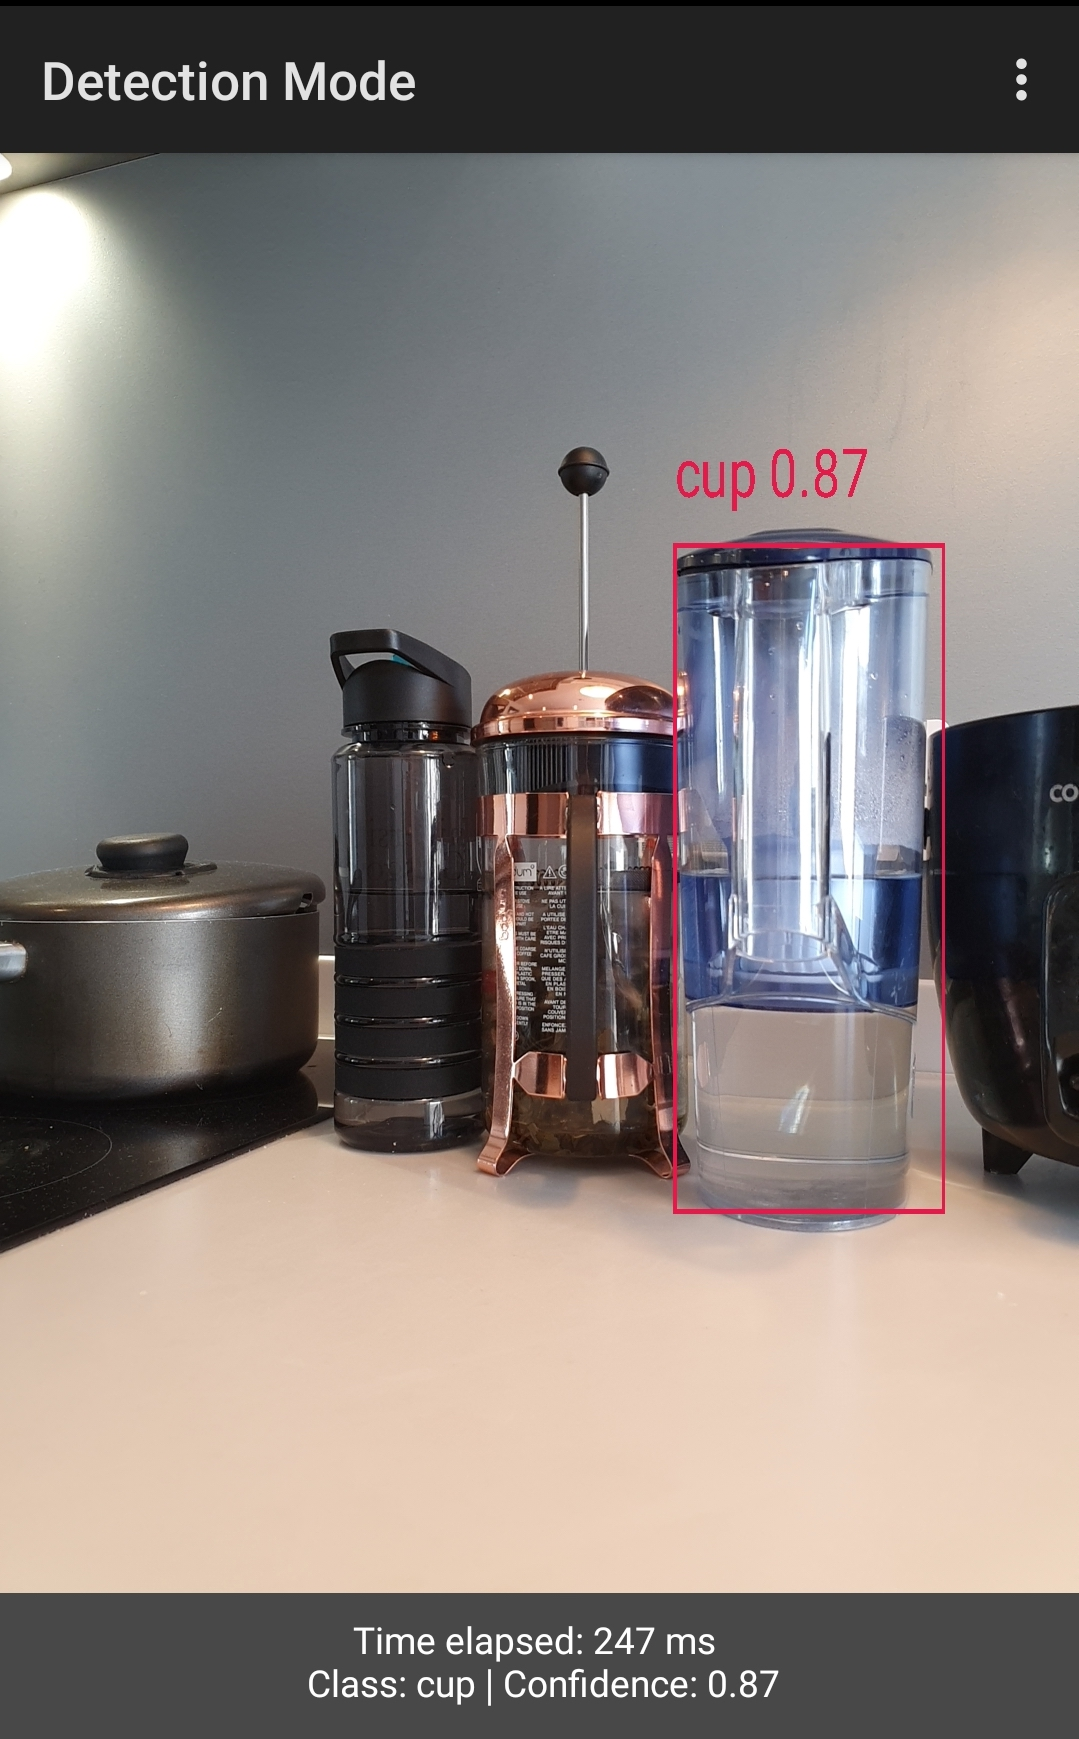
\includegraphics[width=3in]{images/chapter2/object-detector.jpg}
                \caption{Object Detector}
                \label{obj-detector}
            \end{figure}

        \subsection{TensorFlow Object Detection}
            - Model: MobileNet SSD
            - Live Camera: Yes
            - Native Library
            - Library TensorFlow

            \begin{figure}[!ht]
                \centering
                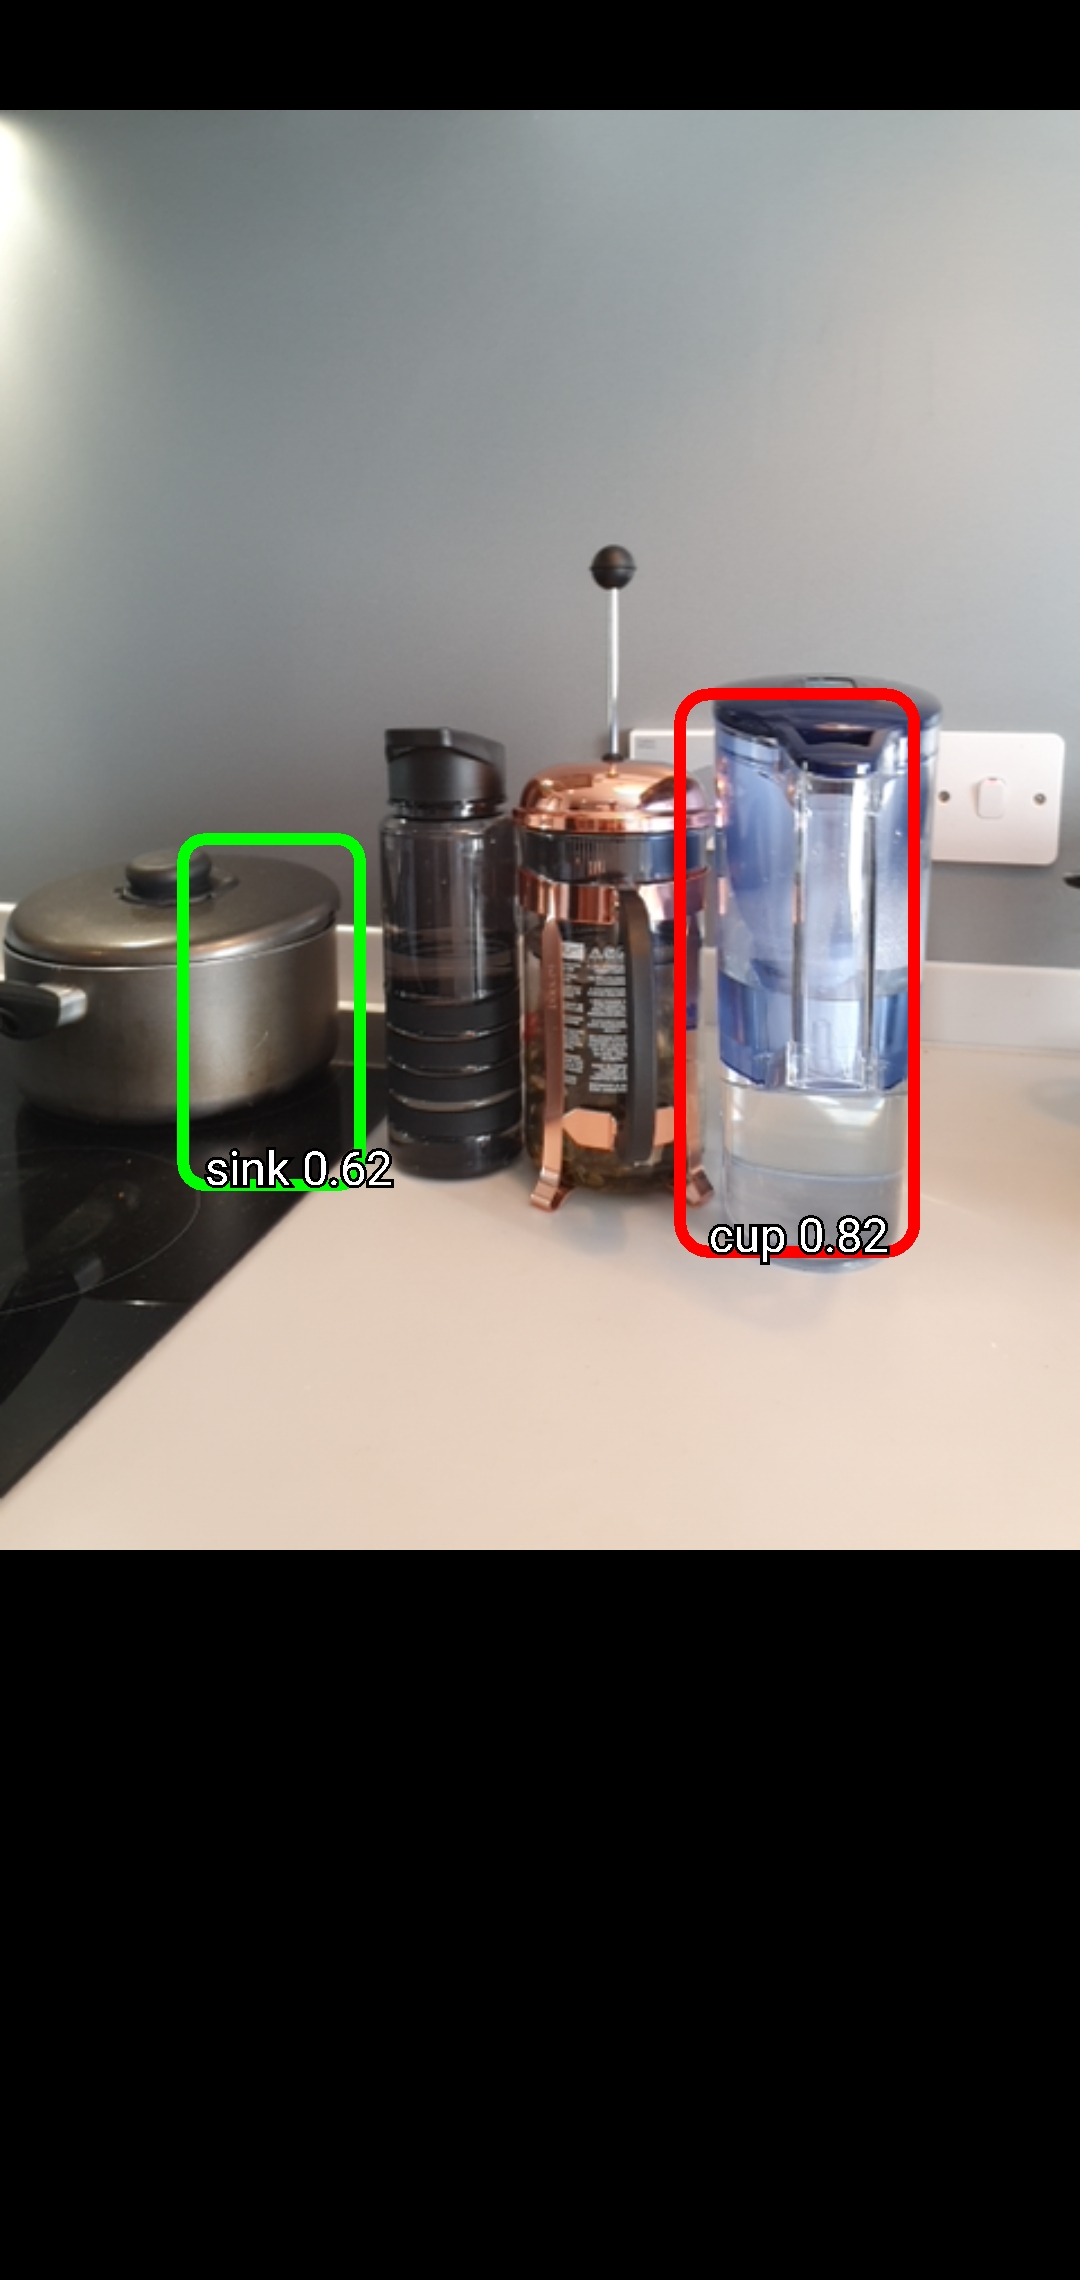
\includegraphics[width=3in]{images/chapter2/ml-detection-tf.jpg}
                \caption{TensorFlow Object Detection}
                \label{ts-obj-detection}
            \end{figure}

        \subsection{Computer Vision Detection}
            - 12 algorithms
                - detect human face
            \begin{figure}[!ht]
                \centering
                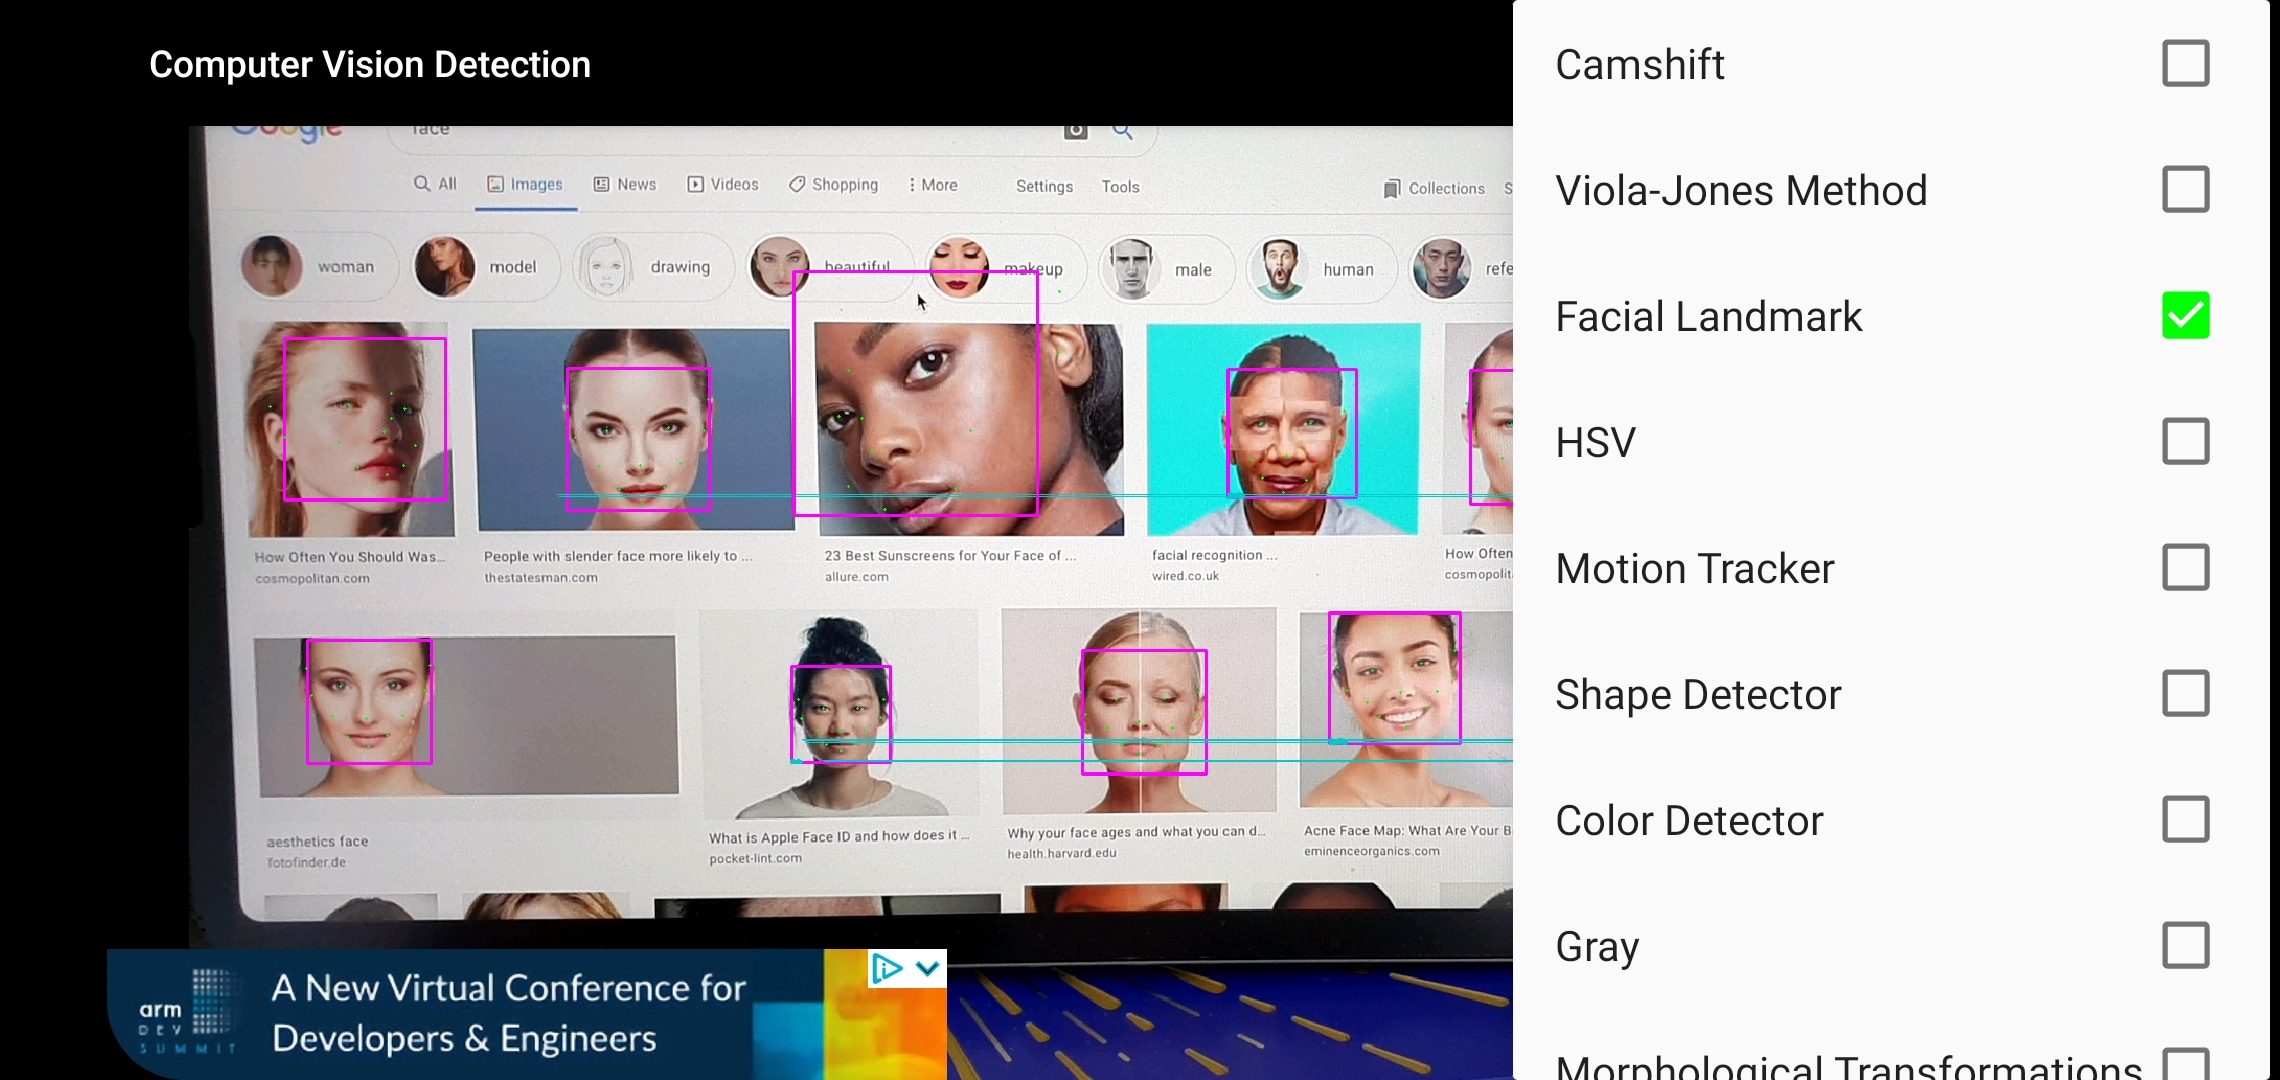
\includegraphics[width=5in]{images/chapter2/cv-detection.jpg}
                \caption{Computer Vision Detection}
                \label{cv-detection}
            \end{figure}

        1.	Object Detector
            -	250-300 ms per frame
            -	Live camera
        2.	Computer Vision Detection
            -	Don’t know about (ms per frame) or (frame per second)
            -	Live camera – not smooth
            -	Lots of features including face detection
            -	Problem is it still delay
